\documentclass[ paper=a4,
                twoside,
                pagesize,
                11pt,
                DIV=10,
                BCOR=10mm,
                cleardoublepage=empty,
                numbers=noenddot,
                titlepage,
                toc=bibliography]{scrartcl}

\newcommand{\sAuthor  }{John Doe}
\newcommand{\sTitle   }{What's in a name?}
\newcommand{\sSubtitle}{An exciting study of names}
\newcommand{\sSubject }{Graduate Seminar on Names \& Origins}
\newcommand{\sCourse  }{Applied Computer Science~(M.Sc.)}
\newcommand{\sNumber  }{24601}
\newcommand{\sDate    }{\today}

% Makes it possible to switch between different languages in the text
% while keeping hyphenation rules correct. Should you add another one
% in the list, please ensure that `english` is the last one. The last
% language is used to control standard hyphenation.
%
% If you write your report in German, you need to change the order.
\usepackage[ngerman,french,english]{babel}
\usepackage[utf8]{inputenc}
\usepackage{csquotes}

%%%%%%%%%%%%%%%%%%%%%%%%%%%%%%%%%%%%%%%%%%%%%%%%%%%%%%%%%%%%%%%%%%%%%%%%
% Bibliography
%%%%%%%%%%%%%%%%%%%%%%%%%%%%%%%%%%%%%%%%%%%%%%%%%%%%%%%%%%%%%%%%%%%%%%%%

\usepackage[%
  autocite     = plain,
  backend      = bibtex,
  doi          = true,
  url          = true,
  giveninits   = true,
  hyperref     = true,
  maxbibnames  = 99,
  maxcitenames = 99,
  sortcites    = true,
  style        = numeric,
  ]{biblatex}

% Remove the month field from the bibliography. It does not serve a good
% purpose, and often, it cannot be used because the journals have crazy
% issue policies.
\AtEveryBibitem{\clearfield{month}}
\AtEveryCitekey{\clearfield{month}}

% Suppress "in" for journal articles.
\renewbibmacro{in:}{%
  \ifentrytype{article}
  {%
  }%
  % else
  {%
    \printtext{\bibstring{in}\intitlepunct}%
  }%
}

% Remove the parentheses for the year in an article. This removes a lot
% of undesired parentheses in the bibliography, which improves
% readability.
\renewbibmacro*{issue+date}{%
  \setunit{\addcomma\space}
    \iffieldundef{issue}
      {\usebibmacro{date}}
      {\printfield{issue}%
       \setunit*{\addspace}%
       \usebibmacro{date}}%
  \newunit}

% Delimit the volume and the number of an article by a colon instead of
% by a dot, which I consider to be more readable.
\renewbibmacro*{volume+number+eid}{%
  \printfield{volume}%
  \setunit*{\addcolon}%
  \printfield{number}%
  \setunit{\addcomma\space}%
  \printfield{eid}%
}

% Do not use a colon for the publisher location. Instead, connect
% publisher, location, and date via commas.
\renewbibmacro*{publisher+location+date}{%
  \printlist{publisher}%
  \setunit*{\addcomma\space}%
  \printlist{location}%
  \setunit*{\addcomma\space}%
  \usebibmacro{date}%
  \newunit%
}

% Ditto for other entry types.
\renewbibmacro*{organization+location+date}{%
  \printlist{location}%
  \setunit*{\addcomma\space}%
  \printlist{organization}%
  \setunit*{\addcomma\space}%
  \usebibmacro{date}%
  \newunit%
}

% Do not abbreviate "technical report".
\DefineBibliographyStrings{english}{%
  techreport = {technical report},
}

% Display the label of a bibliographic entry in bare style, without any
% brackets. I like this more than the default.
%
% This is *really* the proper way of doing this.
\DeclareFieldFormat{labelnumberwidth}{#1\adddot}

% Ensure that DOIs are followed by a non-breakable space.
\DeclareFieldFormat{doi}{%
  \mkbibacro{DOI}\addcolon\addnbspace
    \ifhyperref
      {\href{http://dx.doi.org/#1}{\nolinkurl{#1}}}
      %
      {\nolinkurl{#1}}
}

% Add hair spaces between initials. Technically, this does not amount to
% a large change, but it is typographically correct.
\renewcommand*\bibinitdelim {\addnbthinspace}
\renewcommand*\bibnamedelima{\addnbthinspace}
\renewcommand*\bibnamedelimb{\addnbthinspace}
\renewcommand*\bibnamedelimi{\addnbthinspace}

% Make the font size of citations smaller. This looks more elegant and
% reduces their optical 'weight' somewhat.
\renewcommand*{\citesetup}{%
  \biburlsetup
  \small
}

\bibliography{Seminar}

%%%%%%%%%%%%%%%%%%%%%%%%%%%%%%%%%%%%%%%%%%%%%%%%%%%%%%%%%%%%%%%%%%%%%%%%
% Fonts & colours
%%%%%%%%%%%%%%%%%%%%%%%%%%%%%%%%%%%%%%%%%%%%%%%%%%%%%%%%%%%%%%%%%%%%%%%%

\usepackage[charter]{mathdesign}
\usepackage[oldstyle,scale=0.7]{sourcecodepro}

\usepackage{xcolor}

\definecolor{hd-red}  {RGB}{197, 13, 41}
\definecolor{hd-brown}{RGB}{ 90, 15, 20}
\definecolor{hd-beige}{RGB}{245,240,234}

%%%%%%%%%%%%%%%%%%%%%%%%%%%%%%%%%%%%%%%%%%%%%%%%%%%%%%%%%%%%%%%%%%%%%%%%
% Graphics
%%%%%%%%%%%%%%%%%%%%%%%%%%%%%%%%%%%%%%%%%%%%%%%%%%%%%%%%%%%%%%%%%%%%%%%%

\usepackage{graphicx}
\graphicspath{%
  {Figures/}
  {./}
}

% Suppress warnings about page groups in PDFs. This is not justified
% in most of the cases. I am pretty sure I am including my images in
% the right manner.
\pdfsuppresswarningpagegroup=1

\usepackage{subcaption}

% Make sub-references using \subref being typeset with parentheses.
% Otherwise, only the counter will be printed.
\captionsetup{subrefformat=parens}

% Styling the algorithm captions. They should not be larger than the captions for the figures and
% tables.
\captionsetup[algorithm]{%
  font      = small,
  labelsep  = colon
}

%%%%%%%%%%%%%%%%%%%%%%%%%%%%%%%%%%%%%%%%%%%%%%%%%%%%%%%%%%%%%%%%%%%%%%%%
% TikZ & pgfplots
%%%%%%%%%%%%%%%%%%%%%%%%%%%%%%%%%%%%%%%%%%%%%%%%%%%%%%%%%%%%%%%%%%%%%%%%

\usepackage{tikz}
\usetikzlibrary{%
  arrows,
  backgrounds,
  calc,
  chains,
  colorbrewer,
  decorations.markings,
  intersections,
  positioning,
  shapes
}

\usepackage{pgfplots}
\pgfplotsset{compat=1.14}

% Permits accessing the smallest and largest x value of a plot
\makeatletter
  \newcommand{\pgfplotsxmin}{\pgfplots@xmin}
  \newcommand{\pgfplotsxmax}{\pgfplots@xmax}
\makeatother

% Permits accessing the smallest and largest y value of a plot
\makeatletter
  \newcommand{\pgfplotsymin}{\pgfplots@ymin}
  \newcommand{\pgfplotsymax}{\pgfplots@ymax}
\makeatother

\usepgfplotslibrary{colorbrewer}
\usepgfplotslibrary{colormaps}
\usepgfplotslibrary{external}
\usepgfplotslibrary{fillbetween}
\usepgfplotslibrary{groupplots}
\usepgfplotslibrary{statistics}

%\tikzexternalize
%\tikzsetexternalprefix{Figures/External/}

%%%%%%%%%%%%%%%%%%%%%%%%%%%%%%%%%%%%%%%%%%%%%%%%%%%%%%%%%%%%%%%%%%%%%%%%
% Pseudo-code
%%%%%%%%%%%%%%%%%%%%%%%%%%%%%%%%%%%%%%%%%%%%%%%%%%%%%%%%%%%%%%%%%%%%%%%%
%
% Further information about styling and otherissues with this package is
% available under:
%
% https://tex.stackexchange.com/questions/1375/what-is-a-good-package-for-displaying-algorithms
%

\usepackage{algorithm}
\usepackage{algorithmicx}
\usepackage{algpseudocode}

% Ensures that the `\autoref` command works with algorithms as well. The
% text may have to be changed for other languages, though.
\newcommand{\algorithmautorefname}{Algorithm}

% Use a small font in the body of an algorithm. This removes the weight
% of algorithm environments and makes them typographically more light.
\makeatletter
  \algrenewcommand\ALG@beginalgorithmic{\small}
\makeatother

%%%%%%%%%%%%%%%%%%%%%%%%%%%%%%%%%%%%%%%%%%%%%%%%%%%%%%%%%%%%%%%%%%%%%%%%
% Paragraph lists & compact enumerations
%%%%%%%%%%%%%%%%%%%%%%%%%%%%%%%%%%%%%%%%%%%%%%%%%%%%%%%%%%%%%%%%%%%%%%%%

\usepackage[%
    olditem,  % Do not modify itemize environments by default
    oldenum   % Do not modify enumerate environments by default
  ]{paralist}

%%%%%%%%%%%%%%%%%%%%%%%%%%%%%%%%%%%%%%%%%%%%%%%%%%%%%%%%%%%%%%%%%%%%%%%%
% Typefaces for sections
%%%%%%%%%%%%%%%%%%%%%%%%%%%%%%%%%%%%%%%%%%%%%%%%%%%%%%%%%%%%%%%%%%%%%%%%

\setkomafont{sectioning}{\normalfont\bfseries}
\setkomafont{descriptionlabel}{\normalfont\bfseries}

\setkomafont{caption}{\small}
\setkomafont{captionlabel}{\usekomafont{caption}}

%%%%%%%%%%%%%%%%%%%%%%%%%%%%%%%%%%%%%%%%%%%%%%%%%%%%%%%%%%%%%%%%%%%%%%%%
% Spacing
%%%%%%%%%%%%%%%%%%%%%%%%%%%%%%%%%%%%%%%%%%%%%%%%%%%%%%%%%%%%%%%%%%%%%%%%

\usepackage{setspace}
\onehalfspacing

%%%%%%%%%%%%%%%%%%%%%%%%%%%%%%%%%%%%%%%%%%%%%%%%%%%%%%%%%%%%%%%%%%%%%%%%
% Headers
%%%%%%%%%%%%%%%%%%%%%%%%%%%%%%%%%%%%%%%%%%%%%%%%%%%%%%%%%%%%%%%%%%%%%%%%

\usepackage{scrlayer-scrpage}
\pagestyle{scrheadings}

\lohead{\sAuthor}
\rohead{\sTitle}

%%%%%%%%%%%%%%%%%%%%%%%%%%%%%%%%%%%%%%%%%%%%%%%%%%%%%%%%%%%%%%%%%%%%%%%%
% Tables 
%%%%%%%%%%%%%%%%%%%%%%%%%%%%%%%%%%%%%%%%%%%%%%%%%%%%%%%%%%%%%%%%%%%%%%%%

\usepackage{booktabs}
\usepackage{tabularx}
\usepackage{multirow}

%%%%%%%%%%%%%%%%%%%%%%%%%%%%%%%%%%%%%%%%%%%%%%%%%%%%%%%%%%%%%%%%%%%%%%%%
% Hyperlinks & bookmarks
%%%%%%%%%%%%%%%%%%%%%%%%%%%%%%%%%%%%%%%%%%%%%%%%%%%%%%%%%%%%%%%%%%%%%%%%

\usepackage[%
  colorlinks = true,
  citecolor  = hd-red,
  linkcolor  = hd-red,
  urlcolor   = hd-red,
  ]{hyperref}

\usepackage{bookmark}

%%%%%%%%%%%%%%%%%%%%%%%%%%%%%%%%%%%%%%%%%%%%%%%%%%%%%%%%%%%%%%%%%%%%%%%%
% Proper typesetting of units
%%%%%%%%%%%%%%%%%%%%%%%%%%%%%%%%%%%%%%%%%%%%%%%%%%%%%%%%%%%%%%%%%%%%%%%%

\usepackage[binary-units=true]{siunitx}

\sisetup{%
  detect-all           = true,
  detect-family        = true,
  detect-mode          = true,
  detect-shape         = true,
  detect-weight        = true,
  detect-inline-weight = math,
}

%%%%%%%%%%%%%%%%%%%%%%%%%%%%%%%%%%%%%%%%%%%%%%%%%%%%%%%%%%%%%%%%%%%%%%%%
% Mathematics
%%%%%%%%%%%%%%%%%%%%%%%%%%%%%%%%%%%%%%%%%%%%%%%%%%%%%%%%%%%%%%%%%%%%%%%%

\usepackage{amsmath}
\usepackage{amsthm}
\usepackage{dsfont}

% Fix the spacing of \left and \right. Use these with the proper bracket
% in order to ensure that they scale automatically.
\let\originalleft\left
\let\originalright\right
\renewcommand{\left}{\mathopen{}\mathclose\bgroup\originalleft}
\renewcommand{\right}{\aftergroup\egroup\originalright}

\DeclareMathOperator*{\argmin}          {arg\,min}
\DeclareMathOperator {\dist}            {dist}
\DeclareMathOperator {\im}              {im}

% Proper differential operators
\renewcommand{\d}[1]{\ensuremath{\operatorname{d}\!{#1}}}

% A nice way to typeset proper ordinal superscripts
\newcommand  {\rd}{\textsuperscript{\textup{rd}}\xspace}
\newcommand  {\nd}{\textsuperscript{\textup{nd}}\xspace}
\renewcommand{\th}{\textsuperscript{\textup{th}}\xspace}

%%%%%%%%%%%%%%%%%%%%%%%%%%%%%%%%%%%%%%%%%%%%%%%%%%%%%%%%%%%%%%%%%%%%%%%%
% Penalties
%%%%%%%%%%%%%%%%%%%%%%%%%%%%%%%%%%%%%%%%%%%%%%%%%%%%%%%%%%%%%%%%%%%%%%%%

\clubpenalty         = 10000
\widowpenalty        = 10000
\displaywidowpenalty = 10000

%%%%%%%%%%%%%%%%%%%%%%%%%%%%%%%%%%%%%%%%%%%%%%%%%%%%%%%%%%%%%%%%%%%%%%%%
% Title setup
%%%%%%%%%%%%%%%%%%%%%%%%%%%%%%%%%%%%%%%%%%%%%%%%%%%%%%%%%%%%%%%%%%%%%%%%

\titlehead{%
  \begin{tabular}{ll}
    Name:           & \sAuthor\\
    Course:         & \sCourse\\
    Student number: & \sNumber\\
    Date:           & \sDate\\
  \end{tabular}
}
\subject  {\sSubject}
\author   {\sAuthor}
\title    {\sTitle}
\subtitle {\sSubtitle}
\date     {}

%%%%%%%%%%%%%%%%%%%%%%%%%%%%%%%%%%%%%%%%%%%%%%%%%%%%%%%%%%%%%%%%%%%%%%%%
% Begin of main document
%%%%%%%%%%%%%%%%%%%%%%%%%%%%%%%%%%%%%%%%%%%%%%%%%%%%%%%%%%%%%%%%%%%%%%%%

\begin{document}

  \maketitle

  \tableofcontents
  \bookmarksetup{startatroot}

  %%%%%%%%%%%%%%%%%%%%%%%%%%%%%%%%%%%%%%%%%%%%%%%%%%%%%%%%%%%%%%%%%%%%%%
  % Add your sources here. You may also directly input LaTeX commands
  % here, but the use of `\include` is strongly encouraged.
  %%%%%%%%%%%%%%%%%%%%%%%%%%%%%%%%%%%%%%%%%%%%%%%%%%%%%%%%%%%%%%%%%%%%%%

  \section{Introduction}

This is a simple template for a brief report in a seminar. If you have
used \LaTeX{} before, you should have no trouble accustoming yourself to
it. You may use UTF-8 characters in the document, provided your font supports
them:
%
\begin{quote}
  Allein der Vortrag macht des Redners Glück
\end{quote}
%
The default font in this document supports~(at least) German, French,
and English characters. You should hence have no problem typesetting
complicated names such as \emph{Henri Poincaré} or \emph{Cédric
Villani}. In the following, this document discusses how to typeset
certain things.

\subsection{Typesetting tables}

Tables should be wrapped in a \verb|table| environment and have a proper
caption and label for references. Moreover, typographically correct
lines~(also known as \emph{rules}) should be used. The following example
demonstrates this:
%
\begin{center}
  \begin{verbatim}
    \begin{table}
      \centering
      \begin{tabular}{lSS}
        \toprule
        [...]
        \midrule
        Mount Everest & 8848 & 8848\\
        [...]
        \bottomrule
      \end{tabular}
    \end{table}
    \caption{%
      [...]
    }
    \label{tab:Mountains}
  \end{verbatim}
\end{center}
%
\autoref{tab:Mountains} on \autopageref{tab:Mountains} shows how this
looks in practice.
%
Notice that the \verb|S| column requires additional curly brackets in
order to detect a column heading correctly. If these brackets are
omitted, the heading may not be parsed correctly.

\begin{table}[tb]
  \centering
  \begin{tabular}{lSS}
    \toprule
    \textbf{Mountain}      & \textbf{Height in \si{\meter}} & \textbf{Prominence in \si{\meter}}\\
    \midrule
    Mount Everest & 8848 & 8848\\
    K2            & 8611 & 4020\\
    Kangchenjunga & 8586 & 3922\\
    Lhotse        & 8516 & 610  \\
    \bottomrule
  \end{tabular}
  \caption{
    The highest mountains along with their prominence values.
    %
    This example also demonstrates the use of the \texttt{S} column,
    which permits automatically aligning numbers, as well as the
    \texttt{siunitx} package for typesetting units correctly.
  }
  \label{tab:Mountains}
\end{table}

\subsection{Typesetting figures}

Use the standard \verb|\includegraphics| syntax to include figures. By
default, figures may be specified with their full~(relative) path. You
may also omit a leading \verb|Figures/| folder because \LaTeX{} is going
to automatically look for files in this directory.
%
Notice that specifying the file extension should be unnecessary.
%
\begin{verbatim}
  \begin{figure}[b]
    \centering
    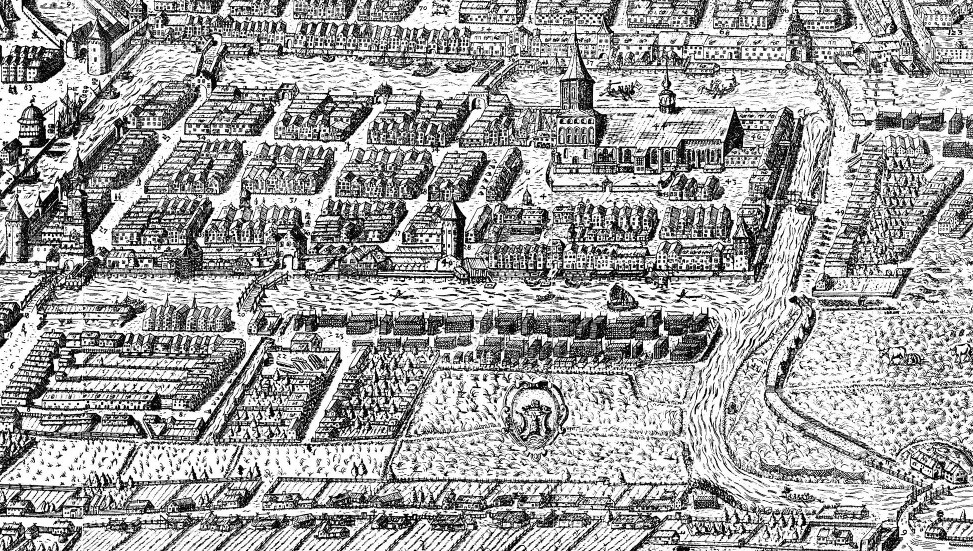
\includegraphics[width=\textwidth]{Koenigsberg}
    \caption{%
      A map of Königsberg from about 1813. Modified from an engraving by
      Joachim Bering from 1613. For annotations, you could use
      \texttt{TikZ} or the \texttt{overpic} package.
    }
    \label{fig:Koenigsberg}
  \end{figure}
\end{verbatim}
%
Figure~\autoref{fig:Koenigsberg} on~\pageref{fig:Koenigsberg} depicts an
example.
%
Please ensure that figures are referenced properly and give credit to
the original author if you use a figure from a publication.
%
You should also check that the resolution of the figure is sufficient.
%
If in doubt, recreate the figure yourself, using \verb|TikZ|\footnote{\url{http://www.texample.net/tikz}}, \verb|pgfplots|\footnote{\url{http://pgfplots.sourceforge.net}}, or any vector graphics application such as \verb|Inkscape|\footnote{\url{https://inkscape.org/en}}.

\begin{figure}[t]
  \centering
  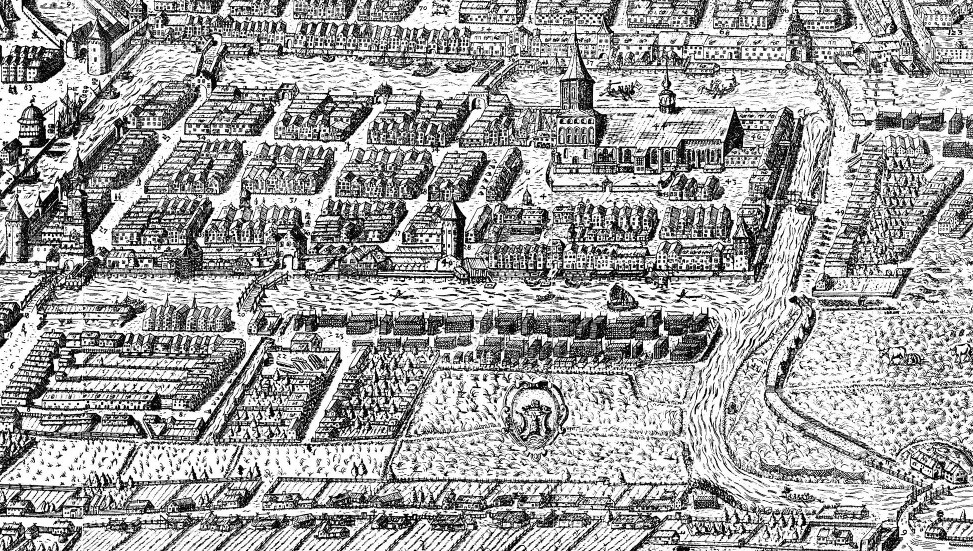
\includegraphics[width=\textwidth]{Koenigsberg}
  \caption{%
    A map of Königsberg from about 1813. Modified from an engraving by
    Joachim Bering from 1613. For annotations, you could use
    \texttt{TikZ} or the \texttt{overpic} package.
  }
  \label{fig:Koenigsberg}
\end{figure}

If you want to add multiple subordinate figures under a larger figure,
use the \verb|subcaption| package that is included by default. It is
good practice to use the \verb|\subcaptionbox| command for wrapping
figures. The first parameter to this command is the caption of the
figure. It may remain empty or contain only a \verb|\label| command for
subsequent references. It is possible to refer to the complete
sub-figure using the usual reference commands. If you want to refer to
an individual sub-figure only, use the \verb|\subref| command.
%
\begin{verbatim}
  \begin{figure}
    \centering
    \subcaptionbox{Label\label{sfig:Label}}{%
      \begin{tikzpicture}
        ...
      \end{tikzpicture}
    }
  \end{figure}
\end{verbatim}
%
\autoref{fig:Anscombe's quartet} depicts numerous sub-figures in order
to show all members of Anscombe's quartet. \autoref{sfig:Anscombe's
quartet A} is the first one of these. This figure is also denoted
by~\subref{sfig:Anscombe's quartet A}, although you should use such
a reference only within a caption because it may be confusing to
readers---and by extension, it may also confuse the people who grade
your report.

Please refer to the source code for more information. It also
demonstrates the use of the \verb|pgfplots| package for high-quality
typesetting of statistical graphics. An introduction would go beyond the
scope of this document, though, but this package is highly recommend if
you want your graphics to have a consistent look-and-feel. 

\begin{figure}
  \centering
  \pgfplotsset{%
    Anscombe/.style={%
      axis x line   = bottom,
      axis y line   = left,
      %
      only marks,
      %
      enlargelimits = false,
      xmin          =  3.5,
      xmax          = 20.0,
      ymin          =  4.0,
      ymax          = 13.0,
      %
      width         = 0.5\linewidth,
      height        = 4cm,
    }
  }
  \subcaptionbox{\label{sfig:Anscombe's quartet A}}{%
    \begin{tikzpicture}
      \begin{axis}[Anscombe]
        \addplot[black, mark=*] table {Data/Anscombe_1.txt};
        \addplot[sharp plot, domain={\pgfplotsxmin:\pgfplotsxmax}] { 3 + 0.5*x };
      \end{axis}
    \end{tikzpicture}
  }
  \subcaptionbox{}{%
    \begin{tikzpicture}
      \begin{axis}[Anscombe]
        \addplot[black, mark=*] table {Data/Anscombe_2.txt};
        \addplot[sharp plot, domain={\pgfplotsxmin:\pgfplotsxmax}] { 3 + 0.5*x };
      \end{axis}
    \end{tikzpicture}
  }\\
  \subcaptionbox{}{%
    \begin{tikzpicture}
      \begin{axis}[Anscombe]
        \addplot[black, mark=*] table {Data/Anscombe_3.txt};
        \addplot[sharp plot, domain={\pgfplotsxmin:\pgfplotsxmax}] { 3 + 0.5*x };
      \end{axis}
    \end{tikzpicture}
  }
  \subcaptionbox{}{%
    \begin{tikzpicture}
      \begin{axis}[Anscombe]
        \addplot[black, mark=*] table {Data/Anscombe_4.txt};
        \addplot[sharp plot, domain={\pgfplotsxmin:\pgfplotsxmax}] { 3 + 0.5*x };
      \end{axis}
    \end{tikzpicture}
  }
  \caption{%
    Multiple figures are best shown using the \texttt{subcaption}
    package. Individual figures may be referenced using the
    \texttt{\textbackslash{}subref} command.
    %
    \subref{sfig:Anscombe's quartet A} depicts the first member of Anscombe's
    quartet, a classical data set in statistics.
  }
  \label{fig:Anscombe's quartet}
\end{figure}

\subsection{Typesetting mathematics}

This template uses \verb|amsmath| and \verb|amssymb|, which are the
de-facto standard for typesetting mathematics. Use numbered equations
using the \verb|equation| environment.
%
If you want to show multiple equations and align them, use the
\verb|align| environment:
%
\begin{align}
    V &:= \{ 1, 2, \dots \}\\
    E &:= \big\{ \left(u,v\right) \mid \dist\left(p_u, p_v\right) \leq \epsilon \big\}
\end{align}
%
Define new mathematical operators using \verb|\DeclareMathOperator|. See
the template for some examples. Else, your operator will be typeset
incorrectly. Observe the difference between the incorrect~(left) and
correct~(right) usage: 
%
\begin{equation}
  cos x \neq \cos x
\end{equation}
%
Moreover, this template contains a correct differential operator. Use \verb|\d| to typeset the differential of integrals:
%
\begin{equation}
  f(u) := \int_{v \in \mathds{D}}\dist(u,v)\d{v}
\end{equation}
%
Take a look at the source for more examples. If in doubt, ask the
organizers for help.

The documentation of the \verb|amsmath|
package\footnote{\url{http://mirrors.ctan.org/macros/latex/required/amsmath/amsmath.pdf}}
is also extremely useful.
%
Likewise, the guide by Mark
Tomforde\footnote{\url{https://www.math.uh.edu/~tomforde/MathWriting.pdf}}
contains a variety of useful tips and tricks.
%
Remember that typesetting complicated things takes some time, but is
usually worth the effort because \emph{you} understand it better, and so
the reader might understand it better as well.

\subsection{Typesetting algorithms}

This template suggests using the \verb|algorithmi| package for
typesetting an algorithm.
%
It is customizable and offers sufficient flexibility to cover most usage scenarios. Feel free to use another package, though, or refer to the extensive documentation\footnote{\url{http://mirror.unl.edu/ctan/macros/latex/contrib/algorithmicx/algorithmicx.pdf}}.
%
There's no standard for pseudo-code, so feel free to use any format that
seems acceptable to you. Always use a caption and a label for your algorithm, so that you may refer to it correctly, e.g.\ \autoref{alg:Persistent homology}.

Notice that for most reports, adding specific algorithms should not be
necessary. However, you are free to go the extra mile if you consider
this to improve the report, in particular if you reference the algorithm
numerous times or if the implementation is a large part of the
contribution.

\begin{algorithm}[t]
  \caption{0-dimensional persistent homology calculation}
  \label{alg:Persistent homology}
  %
  \begin{algorithmic}[1]
    \newcommand{\UF}{\texttt{UF}}
    \newcommand{\diagram}{\mathcal{D}}
    \newcommand{\graph}  {\mathcal{G}}
    \newcommand{\weight} {\mathrm{w}}
    %
    \Require A weighted graph $\graph$
    \State $\UF \gets \emptyset$\Comment{Initialize an empty Union--Find structure}
    \State $\diagram \gets \emptyset$\Comment{Initialize an empty persistence diagram}
    \For{every edge $(u,v)\in\graph$ in ascending order of its weight}
      \State $c \gets$  $\UF$\texttt{.Find}($u$)
      \State $c' \gets$ $\UF$\texttt{.Find}($v$)
      \If{$\weight(c) < \weight(c')$}\Comment{$c$ is the older component; merge $c'$ into it}
        \State $\UF$\texttt{.Union}($c'$, $c$)
        \State $\diagram\gets\diagram\cup\big(\weight(c'), \weight(u,v)\big)$
      \Else\Comment{$c'$ is the older component; merge $c$ into it}
        \State $\UF$\texttt{.Union}($c$, $c'$)
        \State $\diagram\gets\diagram\cup\big(\weight(c) , \weight(u,v)\big)$
      \EndIf
    \EndFor
    \State\Return$\diagram$
  \end{algorithmic}
\end{algorithm}

  \section{Adding content}

This source is in a separate file to demonstrate how to \verb|include|
things. It is good style to let a new section begin on a new page. But
you do not have to do this, of course. If you write longer text, make
judicious use of paragraph breaks by adding newlines. For example, this
is the last line of the paragraph.

And now a new paragraph begins. The short indent of the new paragraph
makes it easier for a reader to perceive breaks in the text, but it is
not as harsh to the eye as a completely blank line. Do \emph{not} fiddle
with the indent or with the spacing between paragraphs!

Along with the standard environments, this template offers
\verb|paralist| for lists within paragraphs.
%
Here's a quick example: The American constitution speaks, among others, of
%
\begin{inparaenum}[(i)]
  \item life
  \item liberty
  \item the pursuit of happiness.
\end{inparaenum}
%
When writing a report, you hopefully have all of these.

\subsection{Citations \& bibliography}

Use the \verb|\autocite| command to cite literature. Do \emph{not} use
citations in lieu of nouns. Hence, the following is generally frowned
upon:
%
\begin{quote}
  As~\autocite{Edelsbrunner10} shows, \dots
\end{quote}
%
Instead, use this:
%
\begin{quote}
  As previously shown~\autocite{Edelsbrunner10}, \dots
\end{quote}
%
Or better:
%
\begin{quote}
  As Edelsbrunner and Harer~\autocite{Edelsbrunner10} showed, \dots
\end{quote}
%
You may also use special citation commands for the author names, e.g.\
\verb|\citet| or \verb|\citep|, but this guide prefers typing the author
names yourself.
%
It is also possible to use \verb|\autocites| to cite multiple authors.
So we could also talk about previous work by Edelsbrunner et
al.~\autocites{Edelsbrunner10, Edelsbrunner02}. Citations will be sorted
automatically.

Particular care should be take in order to properly format citations
that you download from somewhere. Even Google Scholar is known to
produce incorrect references.
%
When in doubt, consult the
documentation\footnote{\url{https://en.wikibooks.org/wiki/LaTeX/Bibliography_Management}}.
The bibliography of this template also contains some examples of proper
bibliography usage.

\subsection{Text in other languages}

Since this template uses \verb|babel| to support different languages, you can easily add ``foreign'' text by wrapping it in \verb|otherlanguage|:
%
\begin{quote}
  \begin{otherlanguage*}{ngerman}
    Uns ist in alten Geschichten viel Herrliches erzählt worden:
    von ruhmvollen Helden und ihren schweren Kämpfen, von
    höchstem Glück, von tiefstem Schmerz und von dem Heldenkampf
    der tapferen Burgunden könnt Ihr jetzt eine herrliche
    Geschichte vernehmen.
  \end{otherlanguage*}
\end{quote}
%
This works for all languages that have been used as optional arguments
in the inclusion of the \verb|babel| package. At present, this only
includes English~(the default language) and French:
%
\begin{quote}
  \begin{otherlanguage*}{french}
    Le roi Charles, notre empereur, le Grand, sept ans tous pleins
    est resté dans l'Espagne: jusqu'à la mer il a conquis la terre
    hautaine. Plus un château qui devant lui résiste, plus une muraille
    à forcer, plus une cité, hormis Saragosse, qui est sur une
    montagne. Le roi Marsile la tient, qui n'aime pas Dieu. C'est
    Mahomet qu'il sert, Apollin qu'il prie. Il ne peut pas s'en garder:
    le malheur l'atteindra. 
  \end{otherlanguage*}
\end{quote}
%
You may add other languages as well but should make sure that the main
language of the document is the \emph{last} one that is specified, as it
controls how things like the table of contents are named.

\subsection{Other resources}

Other resources comprise an excellent guide on how to write a seminar
report\footnote{\url{http://gvv.mpi-inf.mpg.de/teaching/how_to_thesis/how_to_write_a_report_slussalek.pdf}},
as well as Donald Knuth's lectures on mathematical
writing\footnote{\url{http://jmlr.csail.mit.edu/reviewing-papers/knuth_mathematical_writing.pdf}},
although this last guide is more relevant for writing about, well,
mathematics. There are also some good starting points about
\emph{writing} papers and \emph{reading} them by Bob
Laramee~\autocites{Laramee10,Laramee11}.


%%%%%%%%%%%%%%%%%%%%%%%%%%%%%%%%%%%%%%%%%%%%%%%%%%%%%%%%%%%%%%%%%%%%%%%%
% Back matter: don't change anything here
%%%%%%%%%%%%%%%%%%%%%%%%%%%%%%%%%%%%%%%%%%%%%%%%%%%%%%%%%%%%%%%%%%%%%%%%

  \bookmarksetup{startatroot}
  \printbibliography

\end{document}
